\subsection{Добавленные объекты}
\subsubsection{Подсистемаы}
\begin{itemize}	
    \item 
\includegraphics[width=0.02\linewidth]{images/ps}
     "<крюКрюгер">
\end{itemize}
\subsubsection{Регистры сведений}
\begin{itemize}\item 	
\includegraphics[width=0.02\linewidth]{images/rs}
    "<крюЦеныНоменклатурыКонтрагентов">
    \begin{figure}[h]
    	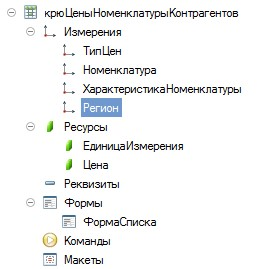
\includegraphics[width=0.4\textwidth]{Rs_priceC.jpg}
    	\caption{Структура регистра.}
    	\label{ris:Rs_priceC.jpg}
    \end{figure}
    
%
\end{itemize}

\subsubsection{Документы}
\begin{itemize}	
    \item 
\includegraphics[width=0.02\linewidth]{images/doc}
%    \todo[fancyline]{Новый док}\textbf{"<крюУстановкаЦенНоменклатурыКонтрагентов">}

	
\end{itemize}

\subsubsection{Константы}
\begin{itemize}	
%	\item 
\includegraphics[width=0.02\linewidth]{images/doc}
	%  \todo[fancyline]{Новый док}\textbf{"<крюУстановкаЦенНоменклатурыКонтрагентов">}
	\item Новая константа "<крюПроверятьЦеныПоставщика">	
	\item Новая константа "<крюПогрешность">	
		
\end{itemize}


%%
\subsubsection{Справочники}
\begin{itemize}	
    \item 
\includegraphics[width=0.02\linewidth]{images/sp}
    "<крюТипыЦенНоменклатурыКонтрагентов">

    \item В справочнике в форме элемента  в  "<ГруппаГлобальныеКоманды">  в "<ПодменюПерейти">  из "<Глобальных команд"> добавлен "<Объект.Ссылка"> справочника "<Типы цен номенклатуры контрагентов"> в подменю появился пункт перехода к "<крюТипыЦенНоменклатурыКонтрагентов">
    
%	\todo[ size=\small,color=blue!40]{Добавить структуру справочника.}%         
	\todo[inline, color=blue!40]{Добавить структуру справочника.}%         
\end{itemize}


\subsection{Измененные объекты}
\marginnote{\Date{Вт.}{12}{Апр.}{2017}}[-40pt]

\subsubsection{Подсистемаы}
\begin{itemize}	
	\item 
\includegraphics[width=0.02\linewidth]{images/ps}
\end{itemize}
\subsubsection{Регистры сведений}
\begin{itemize}\item 	
\includegraphics[width=0.02\linewidth]{images/rs}
\end{itemize}

\subsubsection{Документы}
\begin{itemize}	
	    \item 
\includegraphics[width=0.02\linewidth]{images/doc}
	   	\item В документ "<Поступление ТМЦ"> добавлен реквизит "<НеПроводить">
	   	\item Изменен модуль формы документа, процедура перед записью  и процедура сформировать расхождения 
	   	\item Добавлен макет "<крюРасхождение цен">
\end{itemize}

\subsubsection{Справочники}
\begin{itemize}	
	\item 
\includegraphics[width=0.02\linewidth]{images/sp}
	"<Магазины">
	\begin{itemize}	
		\item В справочник добавлена иерархия
		\sidenote{Для деления по регионам}
		\item В процедуру "<ОбработкаПроверкиЗаполнения"> добавлена проверка группа или элемент - 
		"<Если НЕ ЭтоГруппа Тогда">
	\end{itemize}
    \item В свойствах справочника установлена галка "<Использовать стандартные команды">
\end{itemize}

%\huge\reflectbox{2}2
%WOW
%
%\raisebox{\depth}{\scalebox{1}[-1]{WOW}}
%\recycle

%A\rotatebox{90}{B}C

%Если вы хотите разместить боковую панель с информацией, такой как авторское право и автор, вы можете использовать пакет eso-pic. Пример:

\AddToShipoutPicture{%
	\AtPageLowerLeft{%
%		\hspace*{.02\textwidth}%
		\rotatebox{90}{%

			\begin{minipage}{\paperheight}
				\centering\textcopyright~\today{} ТД Крюгер
			\end{minipage} %
		}
	} %
}%

\menu[,]{Файл, Сохранить как, Item 3, ...}

\directory{Item 1 / Item 2 / Item 3 / ...}

\keys{\Alt 1 + \return + \enter  + ...}

%Если вы используете pdflatex, вы можете создать папку, в которой будут сохраняться все выходные файлы, поэтому ваш верхний каталог будет выглядеть чище.

% в комманды pdflatex -output-directory tmp

%Обратите внимание: папка tmp должна существовать.

	